\documentclass[a4paper]{article}

%\usepackage{fullpage}
\usepackage[14pt]{extsizes}			% размер шрифта
\usepackage[T2A]{fontenc}			% кодировка
\usepackage[utf8]{inputenc}			% кодировка исходного текста
\usepackage[english,russian]{babel}	% локализация и переносы
\usepackage{mathtools}				% математический пакет (включает ams)
\usepackage[thinc]{esdiff}			% производные
\usepackage{graphicx}				% изображения
\usepackage{wrapfig}				% Обтекание рисунков и таблиц текстом
\usepackage{listings}				% програмный код
\lstset{
	numbers=left               
}
\usepackage{setspace}
\onehalfspacing						% полуторный интервал

\usepackage{tocloft}				% точки в содержании для \section
\renewcommand{\cftsecleader}{\cftdotfill{\cftdotsep}}

\author{Бартая Нодари ФМ-101}
\title{ОТЧЁТ\\ Компьютерные технологии в\\ науке и образовании\\ Задание № 5}
\date{\today}

\begin{document}

\begin{titlepage}
	\begin{center}
	Федеральное государственное бюджетное образовательноe учреждение высшего образования \\
	\textbf{«Челябинский государственный университет» \\ (ФГБОУ ВО «ЧелГУ»)}
	\end{center}
	\begin{center}
		Факультет физический			\\
		Кафедра теоретической физики	\\
		Направление 03.04.02 Физика		\\
		Направленность Теоретическая и математическая физика
	\end{center}
	\vfill
	\begin{center}
		\textbf{ОТЧЁТ}
	\end{center}
	\begin{center}
		\textsc{\textbf{Компьютерные технологии\\ в науке и образовании\\ Задание № 5}}
	\end{center}
	\vfill
	\singlespace
	\begin{flushright}
	\begin{tabular}{r p{0.3\textwidth}l}
		Преподаватель:&	доцент кафедры теор. физики, кандидат физ.-мат.наук 
		
		Хайбрахманов С.А. \\[5pt]
		Студент:&	Бартая Н.В.		\\[5pt]
		Группа:& 	ФМ-101			\\
	\end{tabular}
	\end{flushright}
	\onehalfspacing
	\vfill
	\begin{center}
		Челябинск, 2020	
	\end{center}
\end{titlepage}

%\maketitle
\tableofcontents
\setcounter{page}{2}
\newpage
\section{Постановка задачи}\label{Problem}
Требуется рассчитать траекторию движения электрона в скрещенных
постоянных магнитном и электрическом полях с напряженностями 1 А/м и 100 В/м, соответственно. 
Начальная скорость электрона $\mathbf{v}_0$ направлена перпендикулярно вектору напряженности магнитного поля и составляет 10 см/с.
Геометрия задачи представлена на рисунке ниже. За единицу длины примем сантиметр.

\begin{figure}[h]\label{problem}
	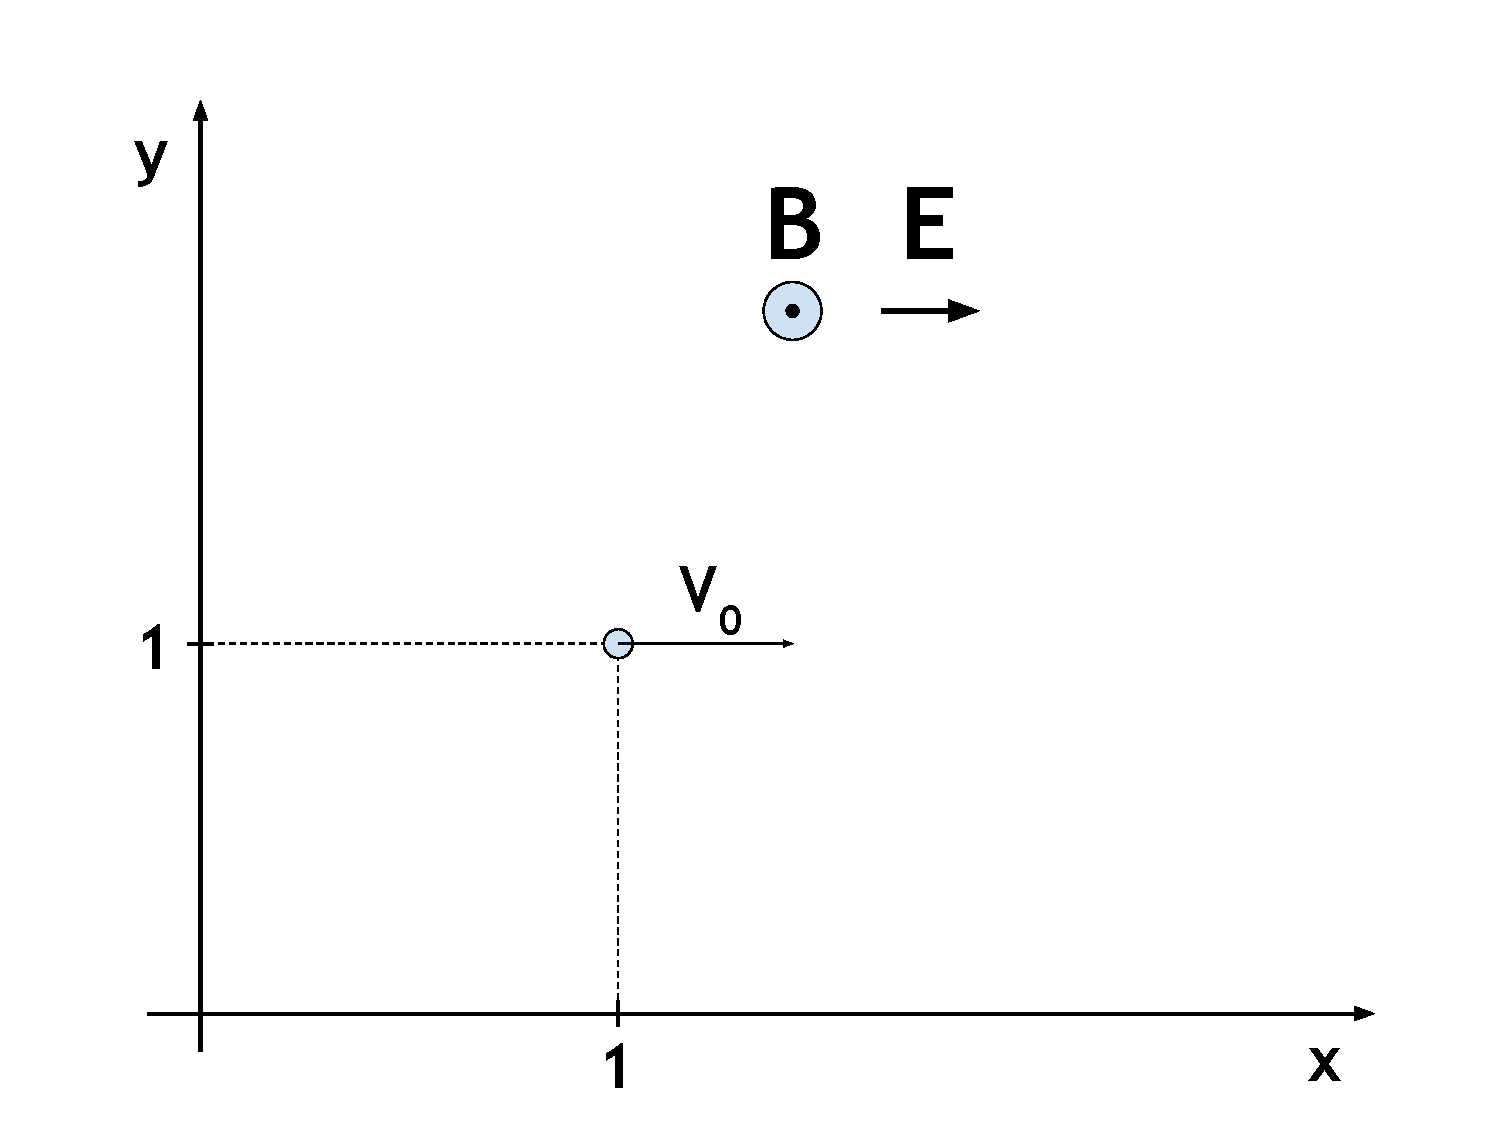
\includegraphics[width=\textwidth]{problem.pdf}
	\caption{Электрон в электромагнитном поле. Показано начальное положение частицы. Электрическое поле направлено вдоль оси $x$, магнитное поле направлено вдоль оси $z$, на наблюдателя. Вектор $\mathbf{v_0}$ показывает направление движения в начальный момент времени.}
\end{figure}

В соответствии с рисунком \ref{problem} введем декартову систему координат, тогда компоненты электрического и магнитного поля будут - $\mathbf{E}=(E_x, 0, 0)$ и $\mathbf{B}=(0, 0, B_z)$, соответственно. Для того, чтобы рассчитать траекторию электрона и его скорость, потребуется уравнение движения, которое, в соответствии со вторым законом Ньютона \cite{Sivukhin:mech} имеет вид:
\begin{equation}\label{motion}
m\diff{\mathbf{v}}{t} = \mathbf{F},
\end{equation}
где $m$ - масса электрона, $\mathbf{v}$ - его скорость, $\mathbf{F}$ - действующая сила.

Известно \cite{Landau:field}, что в элетромагнитном поле на заряженные частицы действует сила Лоренца:
\begin{equation}\label{lorenz}
\mathbf{F} = e \mathbf{E} + \frac{e}{c}\left[\mathbf{vB}\right],
\end{equation}
где $e$ - заряд частицы, $с$ - скорость света, $\mathbf{E}$ и $\mathbf{B}$ - напряженности электрического и магнитного поля, соответственно.

Используя уравнения \eqref{motion} и \eqref{lorenz}, с учётом геометрии задачи \ref{problem} запишем следующую систему уравнений для компонент скоростей движения электрона - 
\begin{equation}\label{v_system}
\begin{cases}
\diff{v_x}{t} = \frac{e}{m}E_x + \frac{e}{cm}\left(v_yB_z\right),	& 	v_x(0) = 10 ; \\[10pt]
\diff{v_y}{t} = -\frac{e}{mc} v_x B_z,					&	v_y(0) = 0 . \\
\end{cases}
\end{equation}
Уравнения для нахождения траектории мы получим из решений системы \eqref{v_system}. Так как по определению \cite{Landau:mech} скорость $\mathbf{v} = d\mathbf{r}/dt$, то уравнения для нахождения координат частиц можно определить, как систему дифференциальных уравнений первого порядка:
\begin{equation}\label{r_system}
\begin{cases}
\diff{r_x}{t} = v_r, 	&	r_x(0) = 1 ;	\\[10pt]
\diff{r_y}{t} = v_y, 	&	r_y(0) = 1.	\\
\end{cases}
\end{equation}
Таким образом у нас имеются все необходимые данные: геометрия задачи \ref{problem} с выбранной системой координат, уравнения и начальные условия \eqref{v_system}, \eqref{r_system} для нахождения скорости движения электрона и его траектории.

\section{Аналитическое решение}
Решение будем искать в нерелятивистском приближении, то есть скорость движения электрона много меньше скорости света. Тогда, согласно второму закону Ньютона уравнение движения электрона имеет вид \cite{Izmaylov} :
\begin{equation}
\diff{m \mathbf{v}}{t} = \dfrac{e}{c} \left[ \mathbf{vB} \right] ,
\end{equation}
что соответствует выведенной ранее системе уравнений \eqref{v_system}. Продифференцируем первое уравнение системы по времени
\[
\diff[2]{v_x}{t} =\frac{e}{cm} B_z \diff{v_y}{t},
\]
введём обозначение $\dfrac{e}{cm}B_z = \gamma$ и подставим второе уравнение вместо $\dot{v_y}$. Получим однородное дифференциальное уравнение второго порядка:
\[
\ddot{v_x} + \gamma^2 v_x = 0 .		
\]
Корни характеристического уравнения оказываются чисто мнимыми и равными ${\lambda_{1,2} = \pm \gamma i}$, следовательно общее решение имеет вид:
\begin{equation}\label{vx_common}
v_x = C_1\, \cos{\gamma t} + C_2\, \sin{\gamma t} .
\end{equation}
Подставим найденное общее решение в уравнение 2 системы \eqref{v_system} и проинтегрируем, следовательно общее решение для $v_y$ имеет вид:
\begin{equation}\label{vy_common}
v_y = C_2 \, \cos{\gamma t} - C_1 \, \sin {\gamma t} + C_3 .
\end{equation}
Продифференцируем по времени общее решение для $v_x$ \eqref{vx_common} и приравняем к первому уравнению системы \eqref{v_system}. В правой части подставим $v_y$ из \eqref{vy_common}. Произведя тривиальные преобразования найдём, что $C_3 = -\xi$, где $\xi = cE_xB_z^{-1}$ Далее, используя начальные условия определим константы - $C_1 = 10$ и $C_2 = \xi$. Таким образом, решением системы уравений \eqref{v_system} будет:
\begin{align}\label{analytic_v}
v_x &= 10 \, \cos{\gamma t} + \xi \sin{\gamma t} , \\
v_y &= \xi \, \cos{\gamma t} - 10 \, \sin {\gamma t} - \xi .
\end{align}
Далее, используя известное решение для компонент $\mathbf{v}$, проинтегрируем оба уравнения из системы \eqref{r_system} как дифференциальные уравнения с разделяющимися переменными, откуда окончательно получаем решение системы \eqref{r_system}:
\begin{align}\label{analytic_r}
%r_x &= \dfrac{10}{\gamma} \sin{\gamma t} - \dfrac{\xi}{\gamma} \cos{\gamma t} + \xi \gamma^{-1} + r_{x0} , \\
%r_y &= \dfrac{\xi}{\gamma} \sin{\gamma t} + \dfrac{10}{\gamma} \cos{\gamma t} - 10 \gamma^{-1} + \xi t  + r_{y0} .
r_x &= \left[10 \, \sin{\gamma t} - \xi \, \cos{\gamma t} + \xi\right] \gamma^{-1} + r_{x0} ,\\
r_y &= \left[\xi \, \sin{\gamma t} + 10 \, \cos{\gamma t} - 10\right] \gamma^{-1} + \xi t  + r_{y0} , 
\end{align} 
где $r_{x0}$ и $r_{y0}$ - координаты частицы в момент времени $t=0$.
%\newpage
\section{Численное решение}
Согласно уравнениям \eqref{motion}, \eqref{lorenz} численное решение для координаты частицы и скорости её движения в зависимости от времени будем искать для следующей системы дифференциальных уравнений первого порядка в соответсвии с геометрией задачи \ref{problem}.
\begin{equation}
	\begin{cases}
		\dot{v_x} = \left[eE_x + \dfrac{e}{c}\left(v_yB_z\right)\right]m^{-1}	
											& 	v_x(0) = 10 \\[10pt]
		\dot{v_y} = -\dfrac{e}{mc} v_x B_z	&	v_y(0) = 0 \\[10pt]
		\dot{r_y} = v_y						&	r_x(0) = 1 \\[10pt]
		\dot{r_y} = v_y						&	r_y(0) = 1 
	\end{cases}
\end{equation}
Данная система решается с помощью модуля integrate \cite{web:scipy.integrate} библиотеки scipy  для языка программирования python. Код программы приведен в разделе \ref{code}. 

На рисунке \ref{graph_t} представлена траектория частицы от начального положения до момента $t = 1$ мкс. На рисункe \ref{graph_s} представлен график зависимости компонент скоростей частицы от времени. Точечными линиями показано аналитическое решение.  Рисунок \ref{graph_m} показывает ошибку численного решения относительно аналитического в разные моменты времени.

Рисунки построены с помощью библиотеки matplotlib \cite{web:matplotlib}.
\begin{figure}
	\centering
	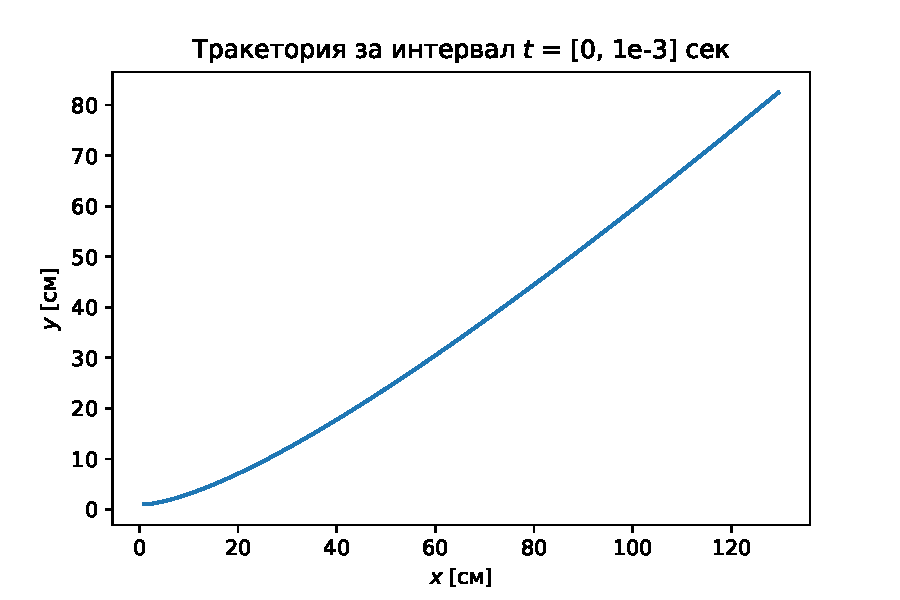
\includegraphics[width=0.8\textwidth]{plotTrajectory.pdf}
	\caption{Траектория частицы за интервал времени $t = [0, 1\text{e-}6]$ сек.}
	\label{graph_t}
\end{figure}

\begin{figure}
	\centering
	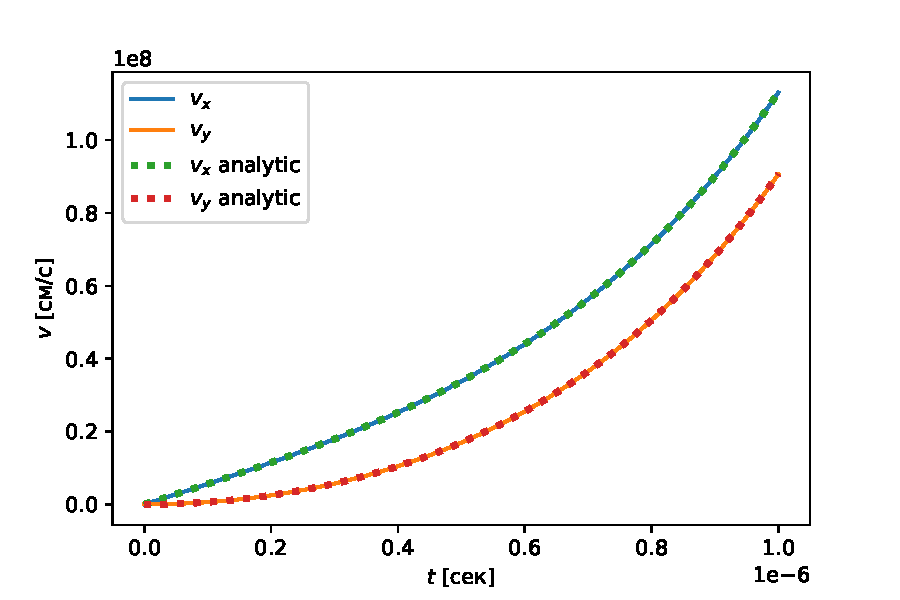
\includegraphics[width=0.8\linewidth]{plotSpeed.pdf}
	\caption{Зависимость компонент скоростей частицы от времени. Сплошные линии - численное решение, прерывистые линии - аналитическое}
	\label{graph_s}
\end{figure}

\begin{figure}
	\centering
	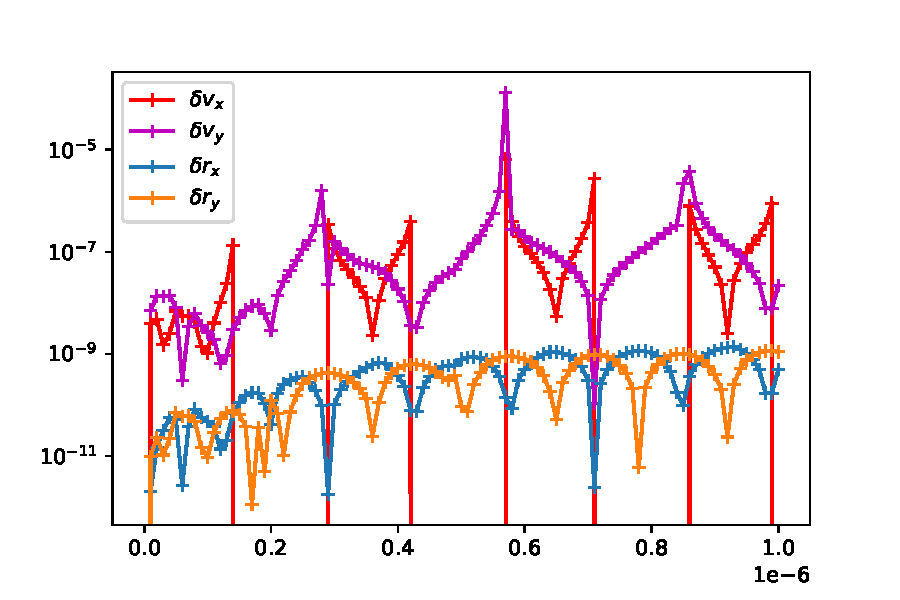
\includegraphics[width=0.8\linewidth]{plotMistake.pdf}
	\caption{График зависимости относительной ошибки численного решения от времени для координат и компонент скоростей частицы. Шкала по оси ординат - логарифмическая.}
	\label{graph_m}
\end{figure}

\section{Заключение}
Поставленная задача выполнена в полном объеме. Аналитическое решение получено в предположении что скорость частицы много меньше скорости света, это справедливо на рассматриваемом временном масштабе. Численное решение получено с помощью средств для языка python,  а именно библиотек scipy\cite{web:scipy}, numpy\cite{web:numpy}. Максимальная относительная погрешность имеет порядок  $1\text{e-}5$ для скоростей частицы и не превышает $1\text{e-}9$ для координат, что является очень хорошим результатом. В целом результаты согласуются с известными ранее (\cite{Landau:field} и др.), что подтверждает правильность полученных аналитических решений и эффективность использования современных средств для решения научных задач.

\clearpage
\section{Код программы}\label{code}
\singlespace
\lstinputlisting[language=Python, firstline=1, lastline=32]{lab5.py}

\onehalfspacing
%\addcontentsline{toc}{chapter}{bibname}
\bibliographystyle{utf8gost705u}  			% стилевой файл для оформления по ГОСТу
\bibliography{biblio}     					% файл библиографической базы 
\addcontentsline{toc}{section}{Список литературы}



\end{document} % Конец текста.